 \documentclass[11pt,a4paper]{article}
\usepackage[utf8]{inputenc}
\usepackage[finnish]{babel}
\usepackage[T1]{fontenc}
\usepackage{amsmath}
\usepackage{amsfonts}
\usepackage{amssymb}
\usepackage{amsthm}
\pagestyle{plain}
\usepackage{graphicx}
\title{Spektometri}
\author{Delun Li\\014631300\\Fysiikan perusopintojen laboratoriotyö\\Työ 12}
\date{20.05.2018}
\begin{document}

\maketitle

\pagebreak

\noindent\Large\textbf{Johdanto}

\vspace{0.5cm}

\noindent Tässä laboratorityössä meidän piti rakentaa spektrometri. Laitteiston avulla pystytään mittaamaan näkyvän valon aallonpituuksia. Meille annettiin määriteltäväksi punaisen ja vihreän valon aallonpituuksia ja vertailla niitä niiden tuntemiin aallonpituuksiin.  

\vspace{0.5cm}

\noindent\Large\textbf{Teoria}

\vspace{0.5cm}

\noindent Tämän työn pohjana käytettiin tunnettua hilayhtälöä, joka kertoo hilan läpi heijastuvan valon aallonpituuden ja kulmat. Interferenssikuvion  havaitaan hilan takanaa olevalla varjostimella, mikä on havainnollistettu alla olevalla kuvalla. 

\vspace{0.3cm}

\noindent Kuva 1: Hilayhtälö

\hspace{2cm}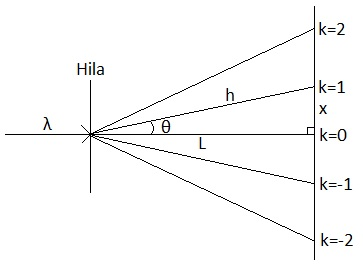
\includegraphics[height=5cm]{Hilayhtalokuva.jpg}

\noindent Kuva siis havannollistaa hilayhtälötä, kuinka valon heijastuminne hilasta varjostimelle teoriassa toimii. Kuvassa kokonaisluvut $K$ kertovat intesiteettimaksimin, jotka näkyvät varjostimella kirkkaina pisteinä. Esimerkiksi kun $k=0$ niin tarkoitetaan, että kyseessä on päämaksimi. Päämaksimi on piste, johon valo osuu heijastumatta hilasta lainkaan. Muille $k$:n arvoille voidaan ilmaista yhälöllä:
\begin{equation}
d sin\theta = k\lambda
\end{equation}

Lausekkeessa $\lambda$ on valon aallopituus ja $d$ on hilavakio. 

Ensimmöisessä intesiteettimaksimissa $k=1$. Kuva 1:ssa nähdään, että $x$ on esimmäisen intesiteettimaksimin etäisyys päämaksimistaj a $L$ on varjostimen etäisyys hilapinnasta. Pythagoran lauseen avulla voidaan sanoa, että $h=\sqrt[]{x^2 + L^2}$, jolloin saadaan lausekkeesta (1) saadaan : 

$$
\lambda = d sin\theta = d\cdot \frac{x}{\sqrt[]{x^2 + L^2}}
$$

Tämän jälkeen on selvitettävä hilavakio $d$ ja sen selvittämiseen voidaan esimerkiksi tutkia sellaisen valon intensiteettimaksimeja, jonka aallonpituus tunnetaan. Meidän tapauksessa käytettiin punaista valoa, jonka aallonpituus $\lambda =645nm$. Tästä siis saadaan laskettua käyttämämme kappalleen hilavakio: 

$$ d=\frac{\sqrt[]{{x_p}^2 + {L_p}^2}\cdot {\lambda}_p}{x_p}$$

Nyt kun tunnettaan hilavakiomme niin voidaan laskea hilayhtälöstämme mielivaltaisen näkyvän valon aallonpituuden kaavalla: 

\begin{equation}
\lambda=\frac{x\cdot d}{\sqrt[]{x^2+L^2}}
\end{equation}


\vspace{0.5cm}

\noindent\Large\textbf{Koejärjestely}

\vspace{0.5cm}

\noindent Ensimmäiseksi haluttiin määrittää hilavakio $d$ punaisen valon avulla. Punaista valoa saatiin käyttämällä laseria, joka tuottaa koherenttia punaista valoa. 

Alla olevassa kuvassa on esitetty laserin sijoitus ja varjostimelle syntyneistä punaisen valon inensiteettimaksimeista. Kuvan oikealla on punaisen laserin lähde, keskellä kiinnitetty CD-levy ja CD-levyn takana valkotaulu. Tässä tapauksessa CD-levy toimii mittauksessa tutkittava hilana ja valkotaulu toimii varjostimena, jossa näkyy syntyneet intensiteettimaksimit. 

\noindent Kuva 2: Punainen valo

\vspace{0.3cm}

\hspace{1.5cm}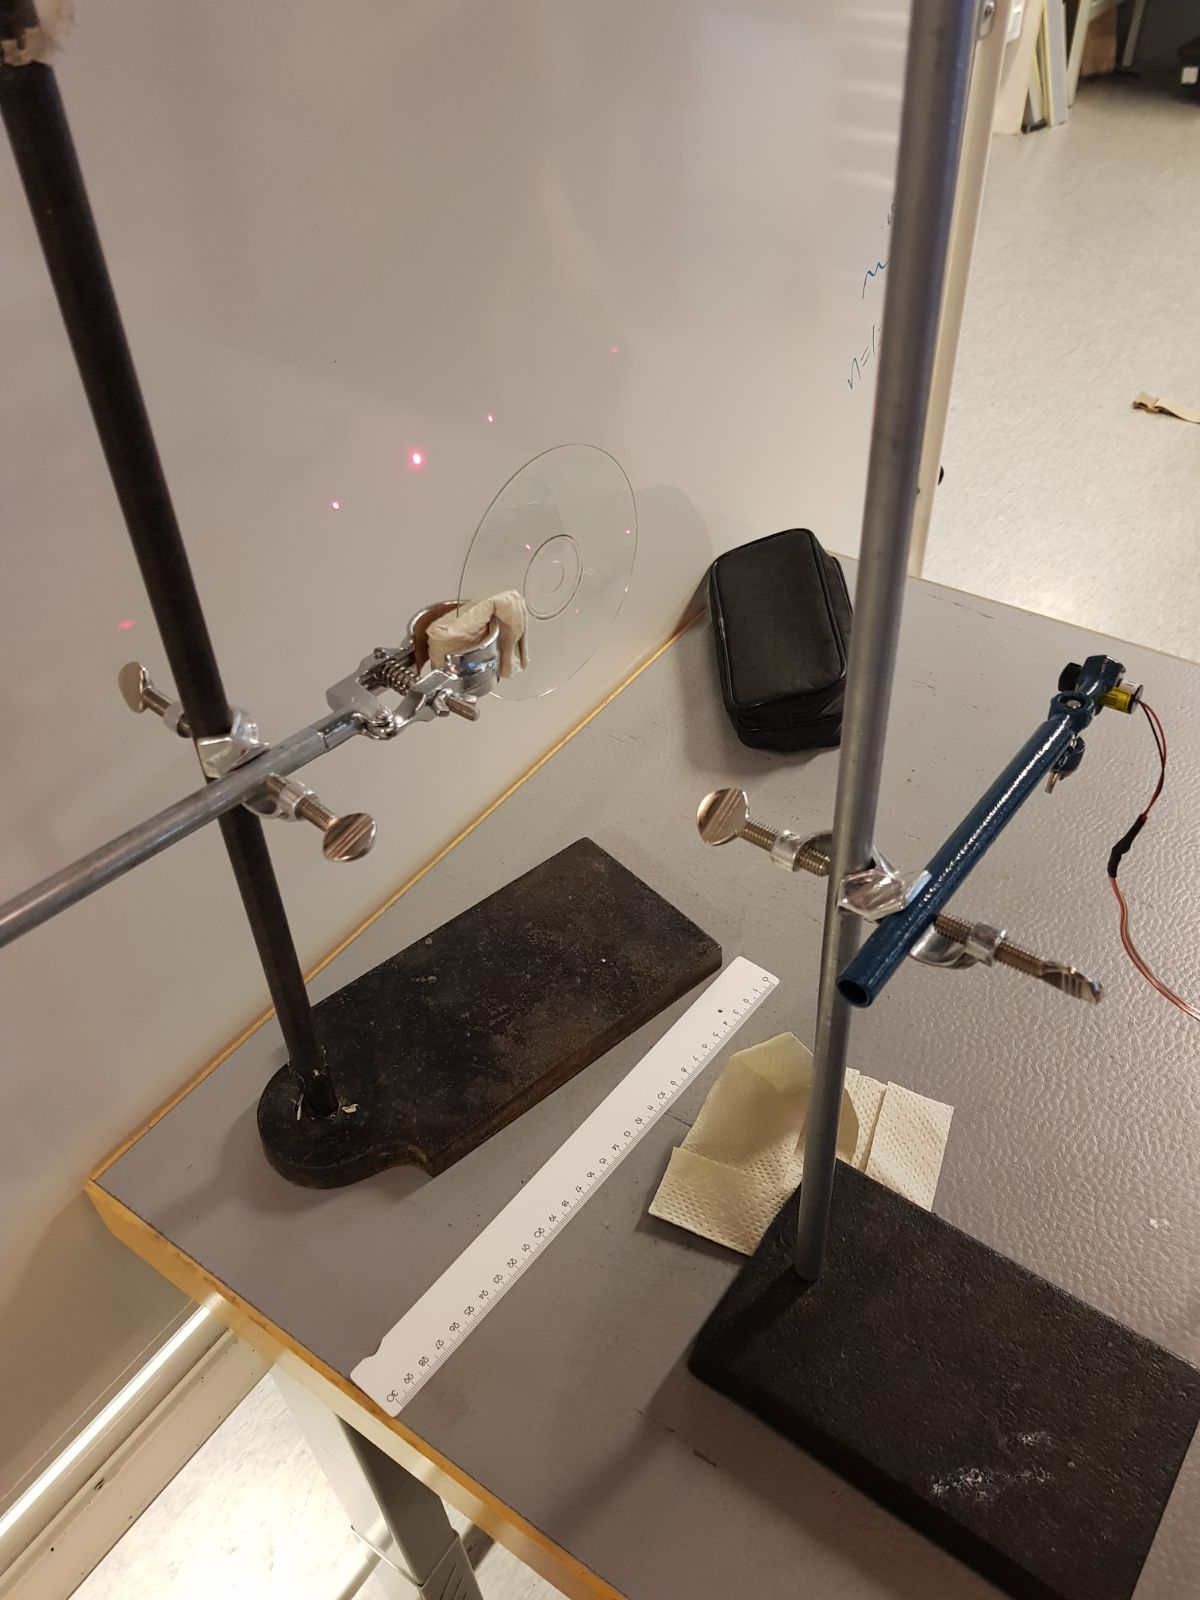
\includegraphics[height=7cm, width=8cm]{3.jpg}

\vspace{0.3cm}

\noindent Punainen laser on koherenttia, jolloin sen etäisyys hilasta ei vaikuta syntyneiden maksimien muotoon. Hilaa asetettiin siten, että ensimmäiset maksimit ovat yhtä etäällä päämaksimista. Kun nämä toetutuvuat, voidaan hyödyntää ja soveltaa hilayhtälöä. Kuvassa näkyy vain päämaksimi ja ensimmäiset maksimit, mutta on olemassa toisia. Tässä tapauksessa ne ovat varjostimen pinnan ulkopuolellä, jolloin niitä ei näe varjostimella. Tässä koejärjestelyssä mitattiin hilan etäisyys varjostimesta ja ensimmäisen maksimin etäisyys päämaksimista. Mittaustulosten avulla voidiin laskea hilavakiolle $d$ arvio. 

Tämän jälkeen tutkittiin vihreää valoa. Vihreä valo saatiin käytössämme olevalta LED-valolta. LEDin tuottama valo ei ole koherenttista valoa, jonka takia koejärjestely tulee olla erilainen. Lähellä hilaa vihreän valon maksimit ilmestyvät paksuina valoympyröinä eikä pistemäisinä. Kaukana hilasta maksimeita ei näy. Tämän takia voidaakseen nähdä vihreän valon maksimeja, meidän oli käytettävä kuperaa linssiä ja LEDin pitää olla kaukana linssistä. Alla oleva kuva esittää vihreän valon taittumisen, joka seuraa linssiyhtälöä eli Gaussin kuvauslakia.

\vspace{0.3cm}

\noindent Kuva 3: Vihreän valon taittuminen 

\vspace{0.3cm}

\hspace{1cm}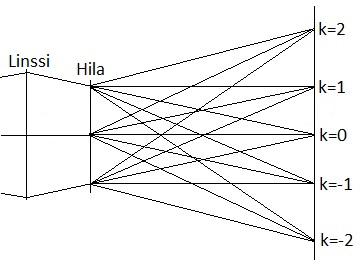
\includegraphics[height=6cm, width=10cm]{Vihreavalo.jpg}

\noindent Kuvasta nähdään, miten valon säteet käyttäytyvät saappuessaan ja taittuessaan linssistäö ja siitä edelleen hilasta. Eli siis linssin avulla saadaan varjostimelle tuttu interferenssikuvio. Nähdään, että jokaisella linssistä taittuvalla valonsäteellä on sama päämaksimi ja samat sivumaskimit. 

Tehtävämme tässä tapauksessa on selvittää vihreän valon aallonpituutta, jolloin riittää tutkia linssistä suoraan kulkevaa valonsädettä ja sen taittumista hilasta. 

Alla olevassa kuvassa on esitettyy vihreän valon sijoittumista ja syntyneret maksimit. Niin kuin ollaan todettu LEDin tulee olla kaukana ja lähellä linssin polttopistettä, jotta saadaan varjostimelle pistemäinen valo. Jos taas liian kaukana hilasta, maksimeja on vaikea havaita tai niitä ei havaita ollenkaan. Kuvasta nähdään myös, että päämaksimin erottaminen on helppoa ja on jo heti vaikeaa havaita ensimmäistä maksimia. 

\pagebreak

\noindent Kuva 4: Vihreä valon koejärjestys

\vspace{0.3cm}

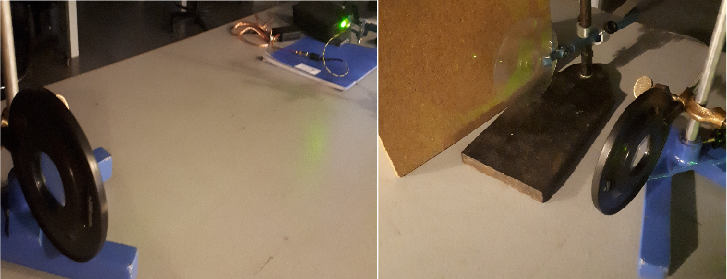
\includegraphics[height=5cm, width=12cm]{2.png}

\vspace{0.5cm}

\noindent\Large\textbf{Tulokset ja tulosten tarkastelu }

\vspace{0.5cm}

\noindent Enimmäiseksi selvitettiin hilavakio $d$ punaisen valon avulla. Tämä laskettiin kaavalla:
$$d=d(x, L)=\frac{\sqrt[]{{x}^2 + {L}^2}\cdot {\lambda}_p}{x} $$

Hilavakio arvion virheen pienentämiseksi suoritettiin toistokokeilla muuttamalla etäisyyksiä. Alla olevaan taulukkoon on koottu mittaustulokset hilavakiolle ja sen virhe on laskettu kaavalla: 
$$\Delta d= \sqrt[]{(\frac{\delta d(x, L)}{\delta x}\cdot \Delta x)^2 + (\frac{\delta d(x, L)}{\delta L}\cdot \Delta L)^2} $$

\vspace{0.3cm}

\noindent Taulukko: Hilavakio 

\vspace{0.3cm}

\hspace{2cm}\begin{tabular}{|c|c|c|c|}
\hline
$L(m)$ & $x(m)$ & $d(nm)$ & $\Delta d(nm)$ \\
\hline
0,128 & 0,062 & 1456,7 & 10,6 \\
\hline
0,135 & 0,065 & 1464,8 & 10,1\\
\hline 
0,190 & 0,091 & 1470,0 & 7,3 \\
\hline
0,195 & 0,094 & 1462,4 & 7,0 \\
\hline
\end{tabular}

\pagebreak

\noindent Taulukon arvojen perusteella ja jättämällä etäisyyksien $x$ ja $L$ aiheuttamat virheet huomioimatta, saadaan hilavakion $d$ keskivarvoksi $d_k = 1463,2nm$, otoskeskihajonnaksi ${\sigma}_d \approx 5,46nm$ ja keskiarvon keskivirheeksi $\delta d_k \approx 2,7nm$. Eli siis hilavakio $d=1463,2nm \pm 2,7nm$

Tämän jälkeen voidaan selvittää vihreän valon aallonpituutta lausekkeella (2), kun vihreän valon voidaan ajatella olevan yksi hilasta taittuva valonsäde: 
$${\lambda}_v={\lambda}_v(x,L,d)=\frac{x\cdot d}{\sqrt[]{x^2+L^2}}$$

\noindent Vihreän valon aallonpituuden virhettä laskettiin kaavalla: 
$$\Delta {\lambda}_v= \sqrt[]{(\frac{\delta {\lambda}_v(x, L,d)}{\delta x}\cdot \Delta x)^2 + (\frac{\delta {\lambda}_v(x, L,d)}{\delta L}\cdot \Delta L)^2 + (\frac{\delta {\lambda}_v(x, L,d)}{\delta d}\cdot \Delta d)^2}
$$

\noindent Tämän jälkeen mitattiin vihreän valon aiheuttamaa päämaksimin keskimääräisen etäisyyden sivumaksimista ja hilan etäisyys varjostimesta. Näiden avulla saadaan arvio vihreän valon aallopituudelle. Alla oleva taulukko esittää mitatut arvot: 

\vspace{0.2cm}

\noindent Taulukko: Vihreä valo 

\vspace{0.3cm}

\hspace{2cm}\begin{tabular}{|c|c|c|c|}
\hline
$L(m)$ & $x(m)$ & ${\lambda}_v (nm)$ & $\Delta {\lambda}_v d(nm)$ \\
\hline
0,050 & 0,0205 & 555,1 & 25,1 \\
\hline
0,060 & 0,0250 & 562,8 & 20,8\\
\hline 
0,073 & 0,0300 & 556,2 & 17,1 \\
\hline

\end{tabular}

\vspace{0.2cm}

\noindent Taulukon avulla saatiiin keskiarvojen keskiarvo vihreän valon aallopituudeksi ${\lambda}_{v,k} \approx 558,0$nm. Saadut arvot vihreän valon aallopiuudelle ovat hyvin lähellä toisiaan ja virheet ovat prosentuaalisesti pienet. 

\noindent Lopuksi tutkittiin millä välillä vihreän ldein aallopituus voi vaihdella. Ledin tapauksessa sivumaksimeilla on leveyttä, jonka takia se vaikeuttaa miittaamista. Ledin aiheuttama leveys johtuu siitä, että vihreä valo sisältää monia aallonpituuksia. Nämä eri aallonpituudet taittuvat hilasta erilailla. Tätä tapausta on havainnollistettu alla olevalla kuvalla.

\vspace{0.2cm}

\noindent Kuva 5: Aallonpituusjakauma 

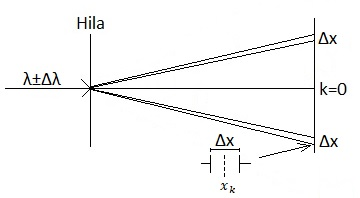
\includegraphics[width=10cm, height=6cm]{Aallonpituusjakauma.jpg}


\noindent Kuva 5 oleva $\Delta \lambda$ kuvaa aallonpituusjakauman ja $\Delta x$ sivumaksimilla havaittu leveys, jonka leveydeksi saatiin $\Delta x \approx 0,003m$. Sivumaksimin reunat ovat $\Delta x/2$ etäisyydellä keskiarvosta. Tämä tarkoittaa, että suuren $x$ virhe on nyt $\Delta x/2 = 0,0015$m arvioidun 1mm sijaan. Nyt kun lasketaan uudella suuren $x$ virherajalla saadaan uudet aallonpituuden virherajat: 

\noindent Taulukko: Vihreän valon aallonpituusjakauma 

\vspace{0.2cm}

\hspace{2cm}\begin{tabular}{|c|c|c|c|}
\hline
$L(m)$ & $x(m)$ & ${\lambda}_v (nm)$ & $\Delta {\lambda}_v d(nm)$ \\
\hline
0,050 & 0,0205 & 555,1 & 36,0 \\
\hline
0,060 & 0,0250 & 562,8 & 29,9\\
\hline 
0,073 & 0,0300 & 556,2 & 24,7 \\
\hline

\end{tabular}

\vspace{0.2cm}

\noindent Talukon avulla saatiin keskiarvon keskiarvoksi edelleen ${\lambda}_{v,k} \approx 558,0$nm ja $\Delta {\lambda}_{v,k} \approx 30,2$nm. Uudesta saadusta arviosta ei ole enään todellinen virhe vaan yliarvio. Mittauksen perusteella vihreän valon aallonpituus on välillä [528,8nm ; 588,2nm] eli ${\lambda}_v = 558,0nm \pm 30,2nm$

\pagebreak

\noindent\Large\textbf{Johtopäätökset}

\noindent Mittauksiemme perusteella saatiin vihreän valon aallonpituudeksi ${\lambda}_v =558$nm. Sivumaksimien leveyden perusteella saatiin vihreälle valolle [528,8nm ; 588,2nm]. Toisaalta todellisuudessa vihreän valon aallonpituus on tavallisesti välillä [490nm ; 560nm] ja keltaisen välillä [560nm ; 590nm]. Näiden perusteella meidän ledin tuottama vihreä valo sisältää pääosin vihreän valon aallonpituuksia ja hieman keltaisen valon aallonpituuksia. Aallonpituuden tarkkuus siis riippuu mittaustarkkuudesta. 

Tästä voidaa päätellä, että jokaiselle valolle pitää etsiä hieman eri sijainti linssille, kuin halutaan mitata muita valon aallonpituuskia. Tämä tehdään, sillä halutaan sivumaksimien näkyvän sopivasti ja helposti mitattavissa. Spektrometrilla voidaan siis miittaa minkä tahansa näkyvän valon aallonpituutta, mutta voi olla hankalaa mitata valoja, joilla on laaja aallonpittusjakauma. Voidaaan siis sanoa, että tällä menetelmällä voidaan helposti selvittää tutkittavan valon aallonpituuden keskiarvo.

\end{document}
